\documentclass[10pt,twocolumn]{article}
\usepackage[margin=0.68in,columnsep=0.22in]{geometry}
\usepackage{amsmath,amssymb,amsthm}
\usepackage{booktabs}
\usepackage{graphicx}
\usepackage{hyperref}
\usepackage{xcolor}
\usepackage{enumitem}

\hypersetup{
  colorlinks=true,
  linkcolor=blue!60!black,
  citecolor=green!45!black,
  urlcolor=blue!65!black,
  pdftitle={Machine-Checked Exact Combinatorial Certificates for Input-Oblivious Unambiguous Hierarchies, Krentel Lex-Max OGTD Collapse, and Single-Query Promise Elimination},
  pdfauthor={Lluis Eriksson}
}

\newtheorem{proposition}{Proposition}
\newtheorem{definition}{Definition}

\newcommand{\ZZ}{\mathbb{Z}}
\newcommand{\NN}{\mathbb{N}}
\newcommand{\OUH}{\mathrm{OUH}}
\newcommand{\OUP}{\mathrm{OUP}}
\newcommand{\ONP}{\mathrm{ONP}}
\newcommand{\SOUP}{\mathrm{SOUP}}
\newcommand{\OGTD}{\mathrm{OGTD}}
\newcommand{\OUGTD}{\mathrm{OUGTD}}
\newcommand{\OUM}{\mathrm{OUM}}

\title{\vspace{-0.8em}\textbf{Machine-Checked Exact Combinatorial Certificates for Input-Oblivious Unambiguous Hierarchies, Krentel Lex-Max OGTD Collapse, and Single-Query Promise Elimination}}
\author{Lluis Eriksson\thanks{Independent researcher; code, Lean~4 proofs, and certificates: MIT license; manuscript and figures: CC-BY-4.0. Prepared with transparent AI assistance via Google Antigravity; all Lean~4 theorems, verifiers, and tests were independently compiled and verified locally. Repository: \url{https://github.com/lluiseriksson/oblivious-unambiguous-hierarchy-certificates}.}}
\date{November 25, 2026}

\begin{document}
\maketitle
\vspace{-1.1em}

\begin{abstract}
Edward A.~Hirsch (\texttt{arXiv:2611.33126}, November 24, 2026) established sharp structural collapses for input-oblivious unambiguous hierarchies built over $\OUP$, proving that the language-oracle hierarchy satisfies $\OUH \subseteq \mathrm{P}^{\mathrm{TALLY}\cap\mathrm{NP}} \subseteq \mathrm{P}_{\|}^{\ONP}$ (Theorem~4.1, Corollary~4.2), that the loose promise-oracle hierarchy collapses into $\OUH^\bullet \subseteq \OGTD[\mathrm{NP}] = \OUGTD[\mathrm{FP}^{\ONP},\mathrm{co}\text{-}\ONP,\mathrm{P}] \subseteq \OUM$ via Krentel lexicographically-largest transcripts (Lemma~3.1, Theorem~5.1), that the oblivious unambiguous dot-operator hierarchy collapses to $\exists^{\mathrm{ou}}\!\cdot\mathrm{co}\text{-}\OUP = \OUP \cup \mathrm{co}\text{-}\OUP$ (Theorem~6.2, Corollary~6.3), that a single loose $\mathrm{prOUP}$ query reduces to an $\OUP$ query ($\OUP^{\mathrm{prOUP}[1]} = \OUP^{\OUP[1]}$, Lemma~6.4, Theorem~6.5), and that $\SOUP = \OUP \cap \mathrm{co}\text{-}\OUP$ (Proposition~6.6). We present a standalone, zero-dependency \textbf{Lean~4.35.0} formalization (\texttt{ObliviousUnambiguousHierarchy.lean}) of 18 finite combinatorial, order-theoretic, and oracle-consistency theorems (0~\texttt{sorry}, 0~warnings, 0~\texttt{Classical.choice}, 11 zero-axiom theorems), paired with a pure-stdlib zero-float finite verifier (\texttt{OUH-CERT-1.0}) auditing four formally specified modes across 16 canonical certificates ($0.038$--$0.789\,\mathrm{ms}$) and rejecting 60/60 live adversarial forgeries.
\end{abstract}

\section{Introduction}
Input-oblivious complexity classes~\cite{fortnow2009fixed,aaronson2014full} restrict nondeterministic witnesses to depend only on the input length~$n$ rather than the individual instance~$x \in \{0,1\}^n$. Combining obliviousness with unambiguity yields $\OUP$, where all positive instances of length~$n$ share a single unique witness $w_n$. Building on the loose unambiguous hierarchy of Hirsch and Sokolov~\cite{hirsch2015unambiguous}, Hirsch~\cite{hirsch2026oblivious} proved that the resulting hierarchies $\OUH$ (language oracles) and $\OUH^\bullet$ (loose promise oracles) collapse dramatically:
\begin{equation}
\begin{aligned}
  \OUH &\subseteq \mathrm{P}^{\mathrm{TALLY}\cap\mathrm{NP}} \subseteq \mathrm{P}_{\|}^{\ONP}, \\
  \OUH^\bullet &\subseteq \OGTD[\mathrm{NP}] \\
  &= \OUGTD[\mathrm{FP}^{\ONP},\mathrm{co}\text{-}\ONP,\mathrm{P}] \subseteq \OUM,
\end{aligned}
  \label{eq:collapses}
\end{equation}
while at the base levels $\exists^{\mathrm{ou}}\!\cdot\mathrm{co}\text{-}\OUP = \OUP \cup \mathrm{co}\text{-}\OUP$, $\OUP^{\mathrm{prOUP}[1]} = \OUP^{\OUP[1]}$, and $\SOUP = \OUP \cap \mathrm{co}\text{-}\OUP$.

\paragraph{Contributions and Explicit Scope.}
We formally verify and audit the \emph{finite combinatorial, order-theoretic, and oracle-consistency core} of~\cite{hirsch2026oblivious}. We explicitly do \emph{not} formalize polynomial-time oracle Turing machines, asymptotic advice polynomials, or uniform circuit encodings inside Lean~4; all complexity-class inclusions remain Hirsch's~\cite{hirsch2026oblivious}:
\begin{enumerate}[leftmargin=*,nosep]
  \item \textbf{Zero-dependency Lean~4 kernel (\S\ref{sec:lean}):} 18 constructive theorems in \texttt{ObliviousUnambiguousHierarchy.lean} (Lean~4.35.0~\cite{demoura2021lean4}), 0~\texttt{sorry}, 0~warnings, 0~\texttt{Classical.choice}, and \textbf{11 zero-axiom theorems}, with every formal signature and inductive predicate stated in Table~\ref{tab:lean}.
  \item \textbf{Pure-stdlib exact verifier (\S\ref{sec:certifier}):} \texttt{OUH-CERT-1.0}, formally specified in Definition~\ref{def:ouhcert}, auditing four finite truth-table modes with zero floating-point arithmetic.
  \item \textbf{Empirical atlas \& red-team audit (\S\ref{sec:results}):} 16 canonical certificates ($0.038$--$0.789\,\mathrm{ms}$ on Windows~11 / Python~3.13), four exact sweeps ($q=2..8$, $h=4..12$, $|\Pi_{\mathrm{out}}|=1..6$), and 60/60 rejected live adversarial forgeries.
\end{enumerate}

\section{Formal Definitions and Combinatorial Core}\label{sec:prelim}

\begin{definition}[Oblivious Classes, Operators, and Pairing~\cite{hirsch2026oblivious}]\label{def:classes}
For length-$n$ inputs $x \in \{0,1\}^n$ and polynomial-length witnesses $w \in \{0,1\}^{p(n)}$:
\begin{itemize}[leftmargin=*,nosep]
  \item $\ONP$ (oblivious $\mathrm{NP}$): $L \in \ONP$ iff a polynomial-time $V$ and length-only advice $w_n$ satisfy $x \in L \iff V(x, w_n)=1$ and $x \notin L \Rightarrow \forall w, V(x,w)=0$. $\mathrm{co}\text{-}\ONP$ is the complement class.
  \item $\OUP$ (oblivious $\mathrm{UP}$): $L \in \OUP$ iff $L \in \ONP$ and on every non-empty slice $L \cap \{0,1\}^n$, $w_n$ is the \emph{unique} $w$ accepted for any $x \in \{0,1\}^n$ (if $L \cap \{0,1\}^n = \emptyset$, no $w$ is accepted). $\mathrm{prOUP}$ is the promise-problem analogue on $\Pi = (\Pi_{\mathrm{YES}}, \Pi_{\mathrm{NO}})$.
  \item $\mathrm{TALLY}$: unary languages over $\{1\}^\ast$. $\SOUP$ (symmetric $\OUP$): $L \in \SOUP$ iff a single unique length-$n$ witness $w_n$ certifies \emph{both} $x \in L$ and $x \notin L$; $\SOUP^{\SOUP}$ denotes $\SOUP$ with a $\SOUP$ oracle.
  \item $\OGTD[\mathcal{C}]$ (oblivious generate-test-decide): $L$ is decided by a triple $(G, T, D)$ with generator $G(1^n)$ outputting advice $a \in \mathrm{Out}_G(n)$, tester $T$ with $\mathrm{Out}_G(n) \subseteq \mathrm{Acc}_T(n)$, and decider $D(x, a) = L(x)$ for all $a \in \mathrm{Acc}_T(n)$. $\OUGTD[\mathcal{F}, \mathcal{T}, \mathcal{D}]$ further enforces $|\mathrm{Acc}_T(n)| \le 1$; $\OUM$ denotes oblivious unambiguous Merlin--Arthur/advice classes containing $\OUGTD[\mathrm{FP}^{\ONP}, \mathrm{co}\text{-}\ONP, \mathrm{P}]$.
  \item Doubled Cantor pairing: $\mathrm{cantor}_2(a, b) := (a+b)(a+b+1) + 2b$ for $a, b \in \NN$, which is injective and satisfies $\mathrm{cantor}_2(a, b) < k(k+1)$ whenever $a + b < k$.
\end{itemize}
\end{definition}

Four exact finite invariants with explicit preconditions drive~\eqref{eq:collapses}:
\begin{enumerate}[leftmargin=*,nosep]
  \item \emph{Tally census \& bit extraction (Lemma~2.8, Theorem~4.1):} Knowing the census count $c_m = |C_m|$ of a finite set $C_m \subseteq \{0,1\}^m$, any subset $S \subseteq C_m$ with $|S| = c_m$ equals $C_m$ uniquely. Given an $\OUP$ verifier~$V$ with unique witness $w_n$ on a non-empty length-$n$ slice, the $p$ parallel tally predicates $W_i \iff \exists x,w: V(x,w)=1 \land w_i=1$ recover $w_n$ bit-for-bit (and return $0^p$ when $L \cap \{0,1\}^n = \emptyset$).
  \item \emph{Krentel lex-max transcript (Lemma~3.1):} Let $G(1^n)$ be a deterministic depth-$q$ adaptive query tree whose $j$-th query depends only on the length-$(j-1)$ answer prefix $a_{<j}$, and let $a^\ast \in \{0,1\}^q$ be the true oracle transcript (so every $0$-bit of $a^\ast$ queries a NO instance). Define $R(a)$ to hold iff every $1$-bit of $a$ queries a YES instance (matching $G(1^n)$ along prefix $a_{<j}$). At the first mismatch index $j$ between any $a \in R$ and $a^\ast$, the prefixes $a_{<j} = a^\ast_{<j}$ issue the identical $j$-th query; since $a^\ast_j = 0$ implies a NO instance whereas $a_j = 1$ certifies a YES instance, necessarily $a_j = 0 < 1 = a^\ast_j$, so $a <_{\mathrm{lex}} a^\ast$. Hence $a^\ast$ is the unique lexicographical maximum of~$R$, recovered in $q$ $\ONP$ prefix probes and uniquely accepted by the $\mathrm{co}\text{-}\ONP$ tester
  \begin{equation}
    T(a) \iff R(a) \;\land\; \forall b \in \{0,1\}^q,\; (a <_{\mathrm{lex}} b \Rightarrow \neg R(b)).
    \label{eq:tester}
  \end{equation}
  \item \emph{Fixed-pair dot-operator collapse (Theorem~6.2):} Suppose $L(x) \iff \exists^{\mathrm{ou}} w \in \{0,1\}^p\, R(x, w)$ ($p \ge 1$) where $\overline{R} \in \OUP$ via verifier $V$ with unique length-oblivious witness $v_N$ ($V((x,w), v) \iff \neg R(x,w) \land v = v_N$). Since at most one $w \in \{0,1\}^p$ satisfies $R(0^n, w)$, at least one of $(0^n, 0^p)$ and $(0^n, 1^p)$ lies in $\overline{R}$. Consequently, the collapsed verifier
  \begin{equation}
  \begin{aligned}
    V'(x, (w, v)) :={}& \bigl(V((0^n,0^p),v) \lor V((0^n,1^p),v)\bigr) \\
    &\land \neg V((x,w),v)
  \end{aligned}
    \label{eq:dotv}
  \end{equation}
  pins $v = v_N$ on anchor $0^n$ and transfers $v_N$ by length-obliviousness to arbitrary $x \in \{0,1\}^n$, forcing $\neg V((x,w), v_N) \iff R(x,w)$ and accepting solely $(w_n, v_N)$.
  \item \emph{Single loose query \& $\SOUP$ tagging (Lemma~6.4, Proposition~6.6):} For a single-query machine $V^O(x,w)$ querying $q(x,w)$ with outcomes $v_0 = V^0(x,w), v_1 = V^1(x,w)$, define the sensitive set $T = \{(x,w) : v_0 \neq v_1\}$. Loose oracle consistency across all extensions $O$ of $\Pi = (\Pi_{\mathrm{YES}}, \Pi_{\mathrm{NO}})$ requires $V^{O_0}(x,w) = V^{O_1}(x,w)$ whenever $q(x,w) \notin \Pi_{\mathrm{YES}} \cup \Pi_{\mathrm{NO}}$, forcing $q(T) \subseteq \Pi_{\mathrm{YES}} \cup \Pi_{\mathrm{NO}}$; insensitive pairs ($v_0 = v_1$) eliminate the query entirely. For $L \in \OUP \cap \mathrm{co}\text{-}\OUP$ with verifiers $Y$ (unique witness $w_Y$ for $L$) and $Z$ (unique witness $w_Z$ for $\overline{L}$), tagging $\mathrm{Tag}(b, w) := (b=1 \land Y(0^n, w)) \lor (b=0 \land Z(0^n, w))$ pins a unique pair $(b^\ast, w^\ast)$ on $0^n$; by length-obliviousness, every $x \in \{0,1\}^n$ is decided using the \emph{same} witness $(b^\ast, w^\ast)$ via $Y(x, w^\ast)$ when $b^\ast = 1$ or $\neg Z(x, w^\ast)$ when $b^\ast = 0$.
\end{enumerate}

\section{Zero-Dependency Lean~4.35.0 Kernel}\label{sec:lean}
We formalize 18 constructive theorems in \texttt{lean/ObliviousUnambiguousHierarchy.lean} (Lean~4.35.0, zero external libraries), audited via \texttt{lean/AuditAxioms.lean} with 0~warnings, 0~\texttt{sorry}, 0~\texttt{Classical.choice}, and 0~\texttt{Lean.ofReduceBool} (11 zero-axiom theorems, Table~\ref{tab:lean}). Auxiliary inductive definitions in the module are:
\begin{itemize}[leftmargin=*,nosep]
  \item $\texttt{cantor2}\;a\;b := (a+b)(a+b+1)+2b$; $\texttt{popcount} : \texttt{List Bool} \to \NN$ counts \texttt{true} entries; $\texttt{BoolSubset}\;s\;c$ holds pointwise on equal-length lists ($s_i=\texttt{true} \Rightarrow c_i=\texttt{true}$).
  \item $\texttt{LexLt}\;a\;b$ is MSB-first strict lexicographic order on equal-length $\texttt{List Bool}$; $\texttt{CertifiedAgainst}\;a\;t$ enforces inductively on equal-length lists that $(a_0=\texttt{true} \Rightarrow t_0=\texttt{true}) \land (a_0=t_0 \Rightarrow \texttt{CertifiedAgainst}\;a'\;t')$.
\end{itemize}

\begin{table*}[t]
\centering
\caption{Complete 18-theorem Lean~4.35.0 kernel in \texttt{ObliviousUnambiguousHierarchy.lean} (0~\texttt{sorry}, 0~warnings, 0~\texttt{Classical.choice}, 11 zero-axiom theorems), listing exact formal signatures and statements.}
\label{tab:lean}
\resizebox{\textwidth}{!}{%
\footnotesize
\setlength{\tabcolsep}{3.0pt}
\begin{tabular}{@{}rllll@{}}
\toprule
\# & Lean~4 Theorem Identifier & Exact Formalized Type / Statement & Ref.~\cite{hirsch2026oblivious} & Axioms \\
\midrule
1 & \texttt{cantor\_pairing\_injective} & $\texttt{cantor2}\;a_1\;b_1 = \texttt{cantor2}\;a_2\;b_2 \Rightarrow a_1=a_2 \land b_1=b_2$ & Lem.~2.8 & \texttt{[p, Q]} \\
2 & \texttt{tally\_census\_subset\_exact} & $\forall s,c:\texttt{List Bool},\; \texttt{BoolSubset}\;s\;c \Rightarrow \texttt{popcount}\;s = \texttt{popcount}\;c \Rightarrow s = c$ & Lem.~2.8 & \texttt{[p, Q]} \\
3 & \texttt{tally\_census\_bit\_determined} & $\texttt{BoolSubset}\;s\;c \Rightarrow \texttt{popcount}\;s = \texttt{popcount}\;c \Rightarrow s[i]? = c[i]?$ & Lem.~2.8 & \texttt{[p, Q]} \\
4 & \texttt{oblivious\_witness\_bit\_extraction} & $V(x_0,w_n) \land (\forall x,w,\,V(x,w)\Rightarrow w=w_n) \Rightarrow ((\exists x,w,\,V(x,w)\land \mathrm{bit}\;w\;i)\iff \mathrm{bit}\;w_n\;i)$ & Thm.~4.1 & \texttt{none} \\
5 & \texttt{oblivious\_empty\_slice\_zero\_witness} & $(\forall x,w,\,\neg V(x,w)) \Rightarrow \neg(\exists x,w,\,V(x,w)\land \mathrm{bit}\;w\;i=\texttt{true})$ & Thm.~4.1 & \texttt{none} \\
6 & \texttt{lex\_max\_transcript\_sound\_and\_unique} & $\forall a,a^\ast:\texttt{List Bool},\; \texttt{CertifiedAgainst}\;a\;a^\ast \Rightarrow a = a^\ast \lor \texttt{LexLt}\;a\;a^\ast$ & Lem.~3.1 & \texttt{[p]} \\
7 & \texttt{prefix\_search\_bit\_recovery} & $(\exists r,\;\texttt{CertifiedAgainst}\;(p+\!\!+\,\texttt{true}::r)\;(p+\!\!+\,b::t)) \iff b = \texttt{true}$ & Lem.~3.1 & \texttt{[p]} \\
8 & \texttt{co\_onp\_tester\_unique\_acceptance} & $|a_1|=|a_2|=q \land T_R(a_1) \land T_R(a_2) \Rightarrow a_1 = a_2$ ($T_R(a) := R(a)\land \forall b,\,a<_{\mathrm{lex}}b\Rightarrow\neg R(b)$) & Lem.~3.1 & \texttt{[p, Q]} \\
9 & \texttt{ogtd\_chain\_inclusion\_sound} & $(\forall a,\,\mathrm{Out}_G\,a\Rightarrow \mathrm{Acc}_T\,a) \land (\forall a,\,\mathrm{Acc}_T\,a\Rightarrow \forall x,\,D\,x\,a=L\,x) \Rightarrow \mathrm{Out}_G\,a \Rightarrow D\,x\,a = L\,x$ & Def.~2.4 & \texttt{none} \\
10 & \texttt{dot\_op\_fixed\_pair\_refutation} & $w_0\neq w_1 \land (\forall u,v,\,R(x_0,u)\Rightarrow R(x_0,v)\Rightarrow u=v) \land \mathrm{Dec}(R(x_0,w_0)) \Rightarrow \neg R(x_0,w_0) \lor \neg R(x_0,w_1)$ & Thm.~6.2 & \texttt{none} \\
11 & \texttt{dot\_op\_collapse\_unique\_witness} & $V\text{-uniq}(v_N) \land (\neg R\Rightarrow V(\cdot,v_N)) \land R\text{-uniq}(w_n) \land \mathrm{Dec}(R) \land V'(x,(w,v)) \Rightarrow w=w_n\land v=v_N$ & Thm.~6.2 & \texttt{none} \\
12 & \texttt{dot\_op\_collapse\_soundness} & $(\neg R(x_0,w_0)\lor\neg R(x_0,w_1)) \land (V(\cdot,v_N)\iff\neg R) \land (L\iff R(\cdot,w_n)) \land \mathrm{Dec} \Rightarrow (L(x)\iff V'(x,(w_n,v_N)))$ & Thm.~6.2 & \texttt{none} \\
13 & \texttt{dot\_op\_union\_distributive} & $(\exists w,\,C(w)\lor D(w)) \iff (\exists w,\,C(w)) \lor (\exists w,\,D(w))$ & Cor.~6.3 & \texttt{none} \\
14 & \texttt{single\_loose\_query\_in\_promise} & $v_0 \neq v_1 \land (\neg P \Rightarrow v_0 = v_1) \land (P \lor \neg P) \Rightarrow P$ & Lem.~6.4 & \texttt{none} \\
15 & \texttt{single\_loose\_query\_insensitive\_elim} & $v_0 = v_1 \Rightarrow \forall b:\texttt{Bool},\; (\text{if }b\text{ then }v_1\text{ else }v_0) = v_0$ & Thm.~6.5 & \texttt{none} \\
16 & \texttt{soup\_shared\_witness\_tag\_exact} & $(Y\iff L\land w=w_Y) \land (Z\iff \neg L\land w=w_Z) \land \mathrm{Dec}(L\,x_0) \Rightarrow \exists!(b^\ast,w^\ast),\;\mathrm{Tag}(b^\ast,w^\ast)$ & Prop.~6.6 & \texttt{none} \\
17 & \texttt{soup\_self\_low\_composition} & $(P_1(w_1)\iff w_1=w_1^\ast) \land (P_2(w_1^\ast,w_2)\iff w_2=w_2^\ast) \Rightarrow (P_1(w_1)\land P_2(w_1,w_2)\iff w_1=w_1^\ast\land w_2=w_2^\ast)$ & Prop.~6.6 & \texttt{none} \\
18 & \texttt{krentel\_transcript\_space\_bounds} & $\forall a,b,k:\NN,\; a + b < k \Rightarrow \texttt{cantor2}\;a\;b < k(k+1)$ & Lem.~2.8 & \texttt{[p, Q]} \\
\bottomrule
\end{tabular}}
\vspace{-0.3em}
\begin{flushleft}
\tiny Axiom key: \texttt{none} = zero axioms (11); \texttt{[p]} = \texttt{[propext]} (2); \texttt{[p, Q]} = \texttt{[propext, Quot.sound]} (5). $\mathrm{Dec}(P)$ denotes explicit decidability hypothesis $P \lor \neg P$.
\end{flushleft}
\vspace{-0.5em}
\end{table*}

\section{Formal Specification of \texttt{OUH-CERT-1.0}}\label{sec:certifier}
The pure-stdlib verifier \texttt{OUH-CERT-1.0} (\texttt{src/ouh\_certifier.py}, \texttt{src/ouh\_exact.py}) uses integer and boolean truth-table arithmetic exclusively, recursively rejecting IEEE-754 floats, booleans-as-integers, unknown keys, duplicate entries, invalid bitstrings, and vacuous witnesses across four formally specified modes:

\begin{definition}[\texttt{OUH-CERT-1.0} JSON Schemas \& Acceptance Predicates]\label{def:ouhcert}
Every certificate contains \texttt{schema="OUH-CERT-1.0"}, \texttt{mode}, \texttt{cert\_id}, and mode-specific fields accepted iff:
\begin{enumerate}[leftmargin=*,nosep]
  \item \textbf{Mode~1 (\texttt{tally\_census\_and\_oblivious\_extraction}):} Given bit-lengths $(n, p)$, universe size $h$, tally bits $C_m \in \{0,1\}^h$, subset $S \subseteq C_m$, and an $\OUP$ truth table $V : \{0,1\}^n \times \{0,1\}^p \to \{0,1\}$, accepts iff $S \subseteq C_m \land |S| = |C_m| \Rightarrow S = C_m$, $\mathrm{cantor}_2$ is injective on claimed pairs, $V$ has at most one accepting witness across all $x$, and bit-by-bit tally extraction recovers $w_n$ (or $0^p$ on empty slices).
  \item \textbf{Mode~2 (\texttt{krentel\_lex\_max\_ogtd\_cert}):} Given adaptive query depth $q \in [2, 8]$, explicit prefix-deterministic query map $Q : \{0,1\}^{<q} \to U$, and NP-oracle indicator $O : U \to \{0,1\}$, exhaustively enumerates all $2^q$ transcripts, computes $R = \{a : \forall j, a_j=1 \Rightarrow O(Q(a_{<j}))=1\}$, and accepts iff $a^\ast = \max_{\mathrm{lex}} R$, all $q$ prefix probes match $a^\ast$, and $|\{a : T(a)\}| = 1$ under~\eqref{eq:tester}.
  \item \textbf{Mode~3 (\texttt{dot\_operator\_collapse\_exact}):} Given $(n, p, r)$ ($p \ge 1$) and finite truth tables for $R(x,w)$ and inner $\OUP$ verifier $V((x,w), v)$ for $\overline{R}$, accepts iff $V$ accepts solely $v_N$ on $\overline{R}$, $R$ accepts at most one $w_n$, $(0^n,0^p) \in \overline{R} \lor (0^n,1^p) \in \overline{R}$, and $V'$ in~\eqref{eq:dotv} accepts solely $(w_n, v_N)$ for $x \in L$.
  \item \textbf{Mode~4 (\texttt{single\_loose\_query\_and\_soup\_exact}):} Given promise partition $(\Pi_{\mathrm{YES}}, \Pi_{\mathrm{NO}}, \Pi_{\mathrm{out}})$, single-query verifier $(q(x,w), V^0, V^1)$, and complementary $\OUP$ verifiers $(Y, Z)$ for $(L, \overline{L})$, exhaustively replays all $2^{|\Pi_{\mathrm{out}}|}$ consistent oracle extensions $O$, accepting iff $V^O$ is consistent across all extensions, $q(T) \subseteq \Pi_{\mathrm{YES}} \cup \Pi_{\mathrm{NO}}$, insensitive pairs eliminate the query, and $\mathrm{Tag}(b, w)$ on $0^n$ yields a unique shared witness $(b^\ast, w^\ast)$ deciding all $x \in \{0,1\}^n$.
\end{enumerate}
\end{definition}

\section{Empirical Atlas and Red-Team Audit}\label{sec:results}
Running \texttt{scripts/run\_all\_experiments.py} (Windows~11, Python~3.13 pure-stdlib) produces 16 canonical certificates (4 per mode) and four exact combinatorial sweeps, audited end-to-end by \texttt{scripts/verify\_all.py} with SHA-256 verification across all 41 tracked repository files.

\begin{figure}[t]
  \centering
  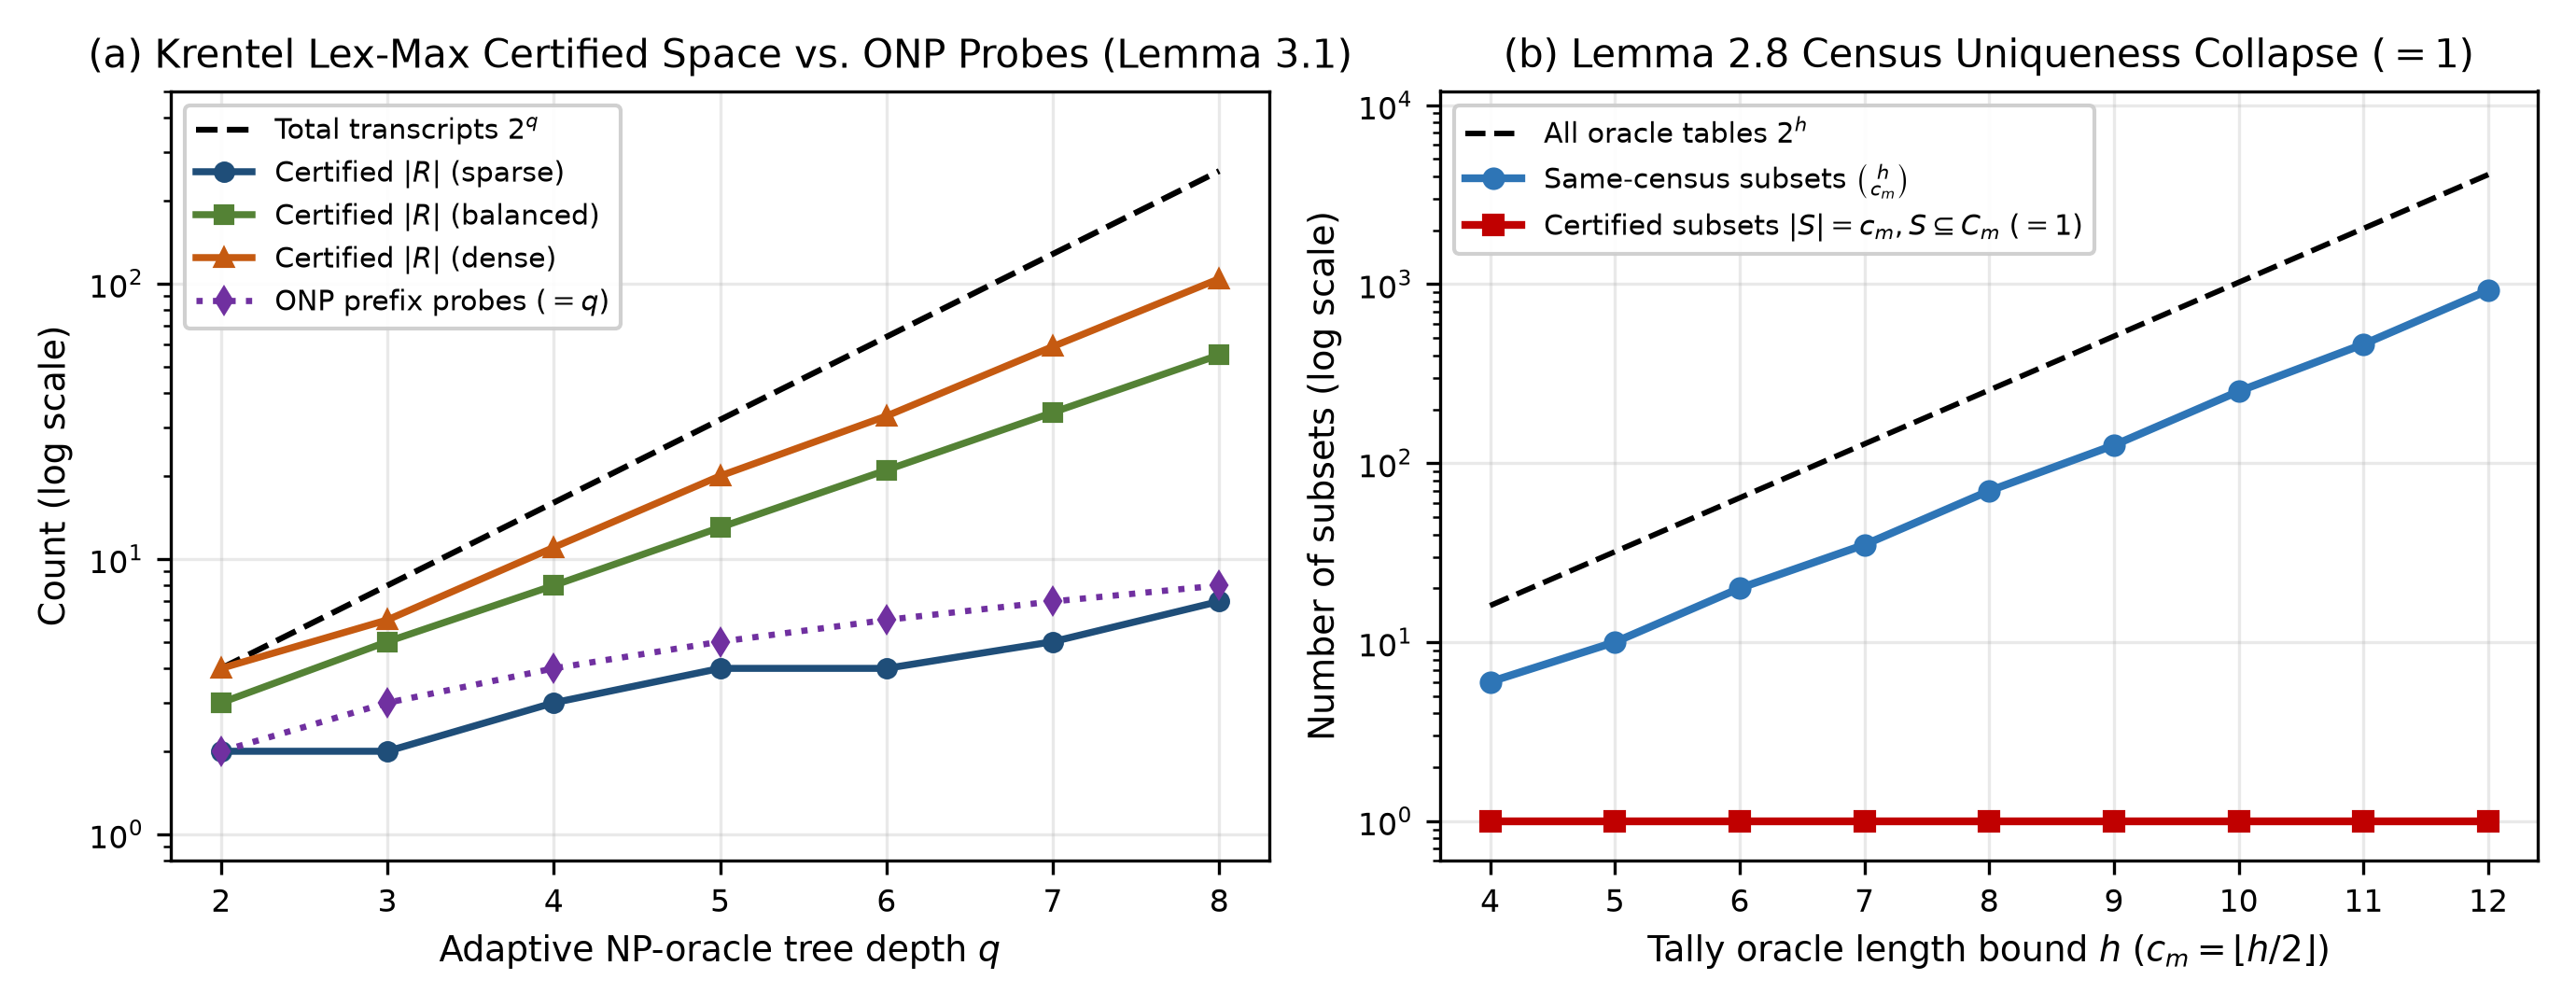
\includegraphics[width=\columnwidth]{../figures/fig1_krentel_ogtd_and_tally_census.png}
  \caption{(a) Exact Lemma~3.1 Krentel certified transcript count $|R|$ across depths $q=2\dots 8$ (sparse, balanced, dense regimes) versus $2^q$ total transcripts and $q$ $\ONP$ prefix probes. (b) Exact Lemma~2.8 tally-census collapse from $\binom{h}{c_m}$ same-size subsets to exactly~$1$ certified subset ($h=4\dots 12$).}
  \label{fig:krentel}
\end{figure}

\paragraph{Krentel Transcripts and Tally Census (Fig.~\ref{fig:krentel}).}
Across adaptive depths $q=2\dots 8$ ($2^q = 4\dots 256$), $|R|$ spans $7$ (sparse), $55$ (balanced), and $104$ (dense) transcripts at $q=8$, yet in 100\% of instances $\ONP$ prefix search recovers $a^\ast$ in $q$ probes and tester~\eqref{eq:tester} achieves $|\mathrm{Acc}_T|=1$. In Mode~1 ($0.038$--$0.084\,\mathrm{ms}$), exact bit-by-bit tally extraction recovers both non-empty witnesses (up to $n=4, p=6$, $|L|=11$) and empty-slice $0^5$, while census uniqueness collapses $\binom{12}{6} = 924$ same-size subsets (out of $2^{12}=4096$) to~$1$.

\begin{figure}[t]
  \centering
  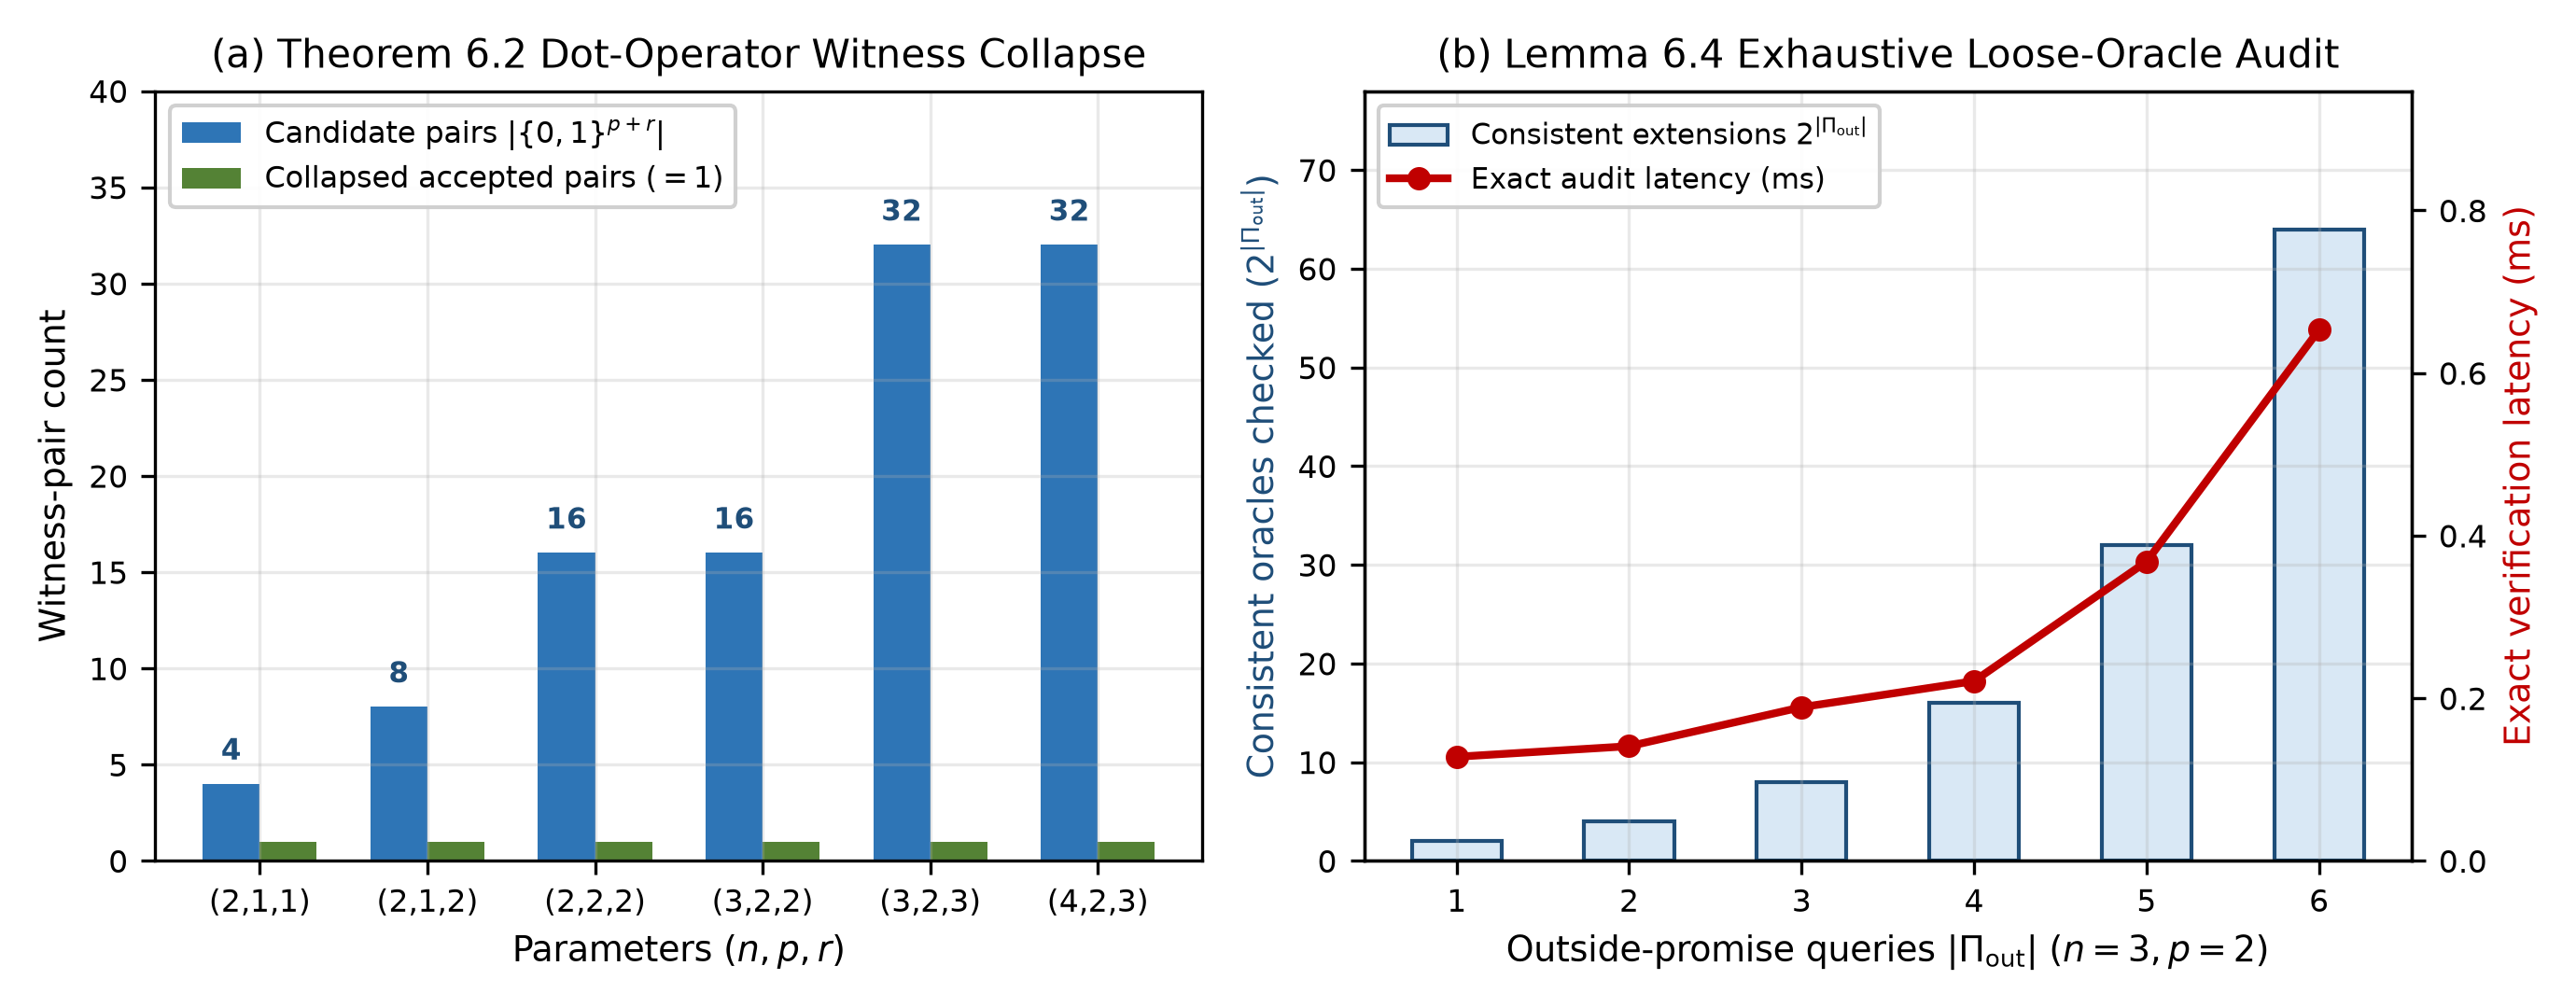
\includegraphics[width=\columnwidth]{../figures/fig2_dot_collapse_and_loose_promise.png}
  \caption{(a) Theorem~6.2 dot-operator collapse across $(n,p,r)$: fixed-pair refutation collapses $2^{p+r}$ candidate pairs to exactly~$1$ unique witness $(w_n,v_N)$. (b) Exhaustive Lemma~6.4 loose-oracle audit across $|\Pi_{\mathrm{out}}|=1\dots 6$ ($2\dots 64$ consistent extensions, $0.128$--$0.653\,\mathrm{ms}$).}
  \label{fig:collapse}
\end{figure}

\paragraph{Dot Collapse, Loose Extensions, and $\SOUP$ (Fig.~\ref{fig:collapse}).}
In Mode~3 ($0.068$--$0.183\,\mathrm{ms}$), fixed-pair refutation collapses up to $2^{2+3}=32$ witness pairs to $(w_n,v_N)$ at $(n,p,r)=(4,2,3)$ ($|L|=9$). In Mode~4 ($0.117$--$0.789\,\mathrm{ms}$), exhaustive auditing across up to $2^5 = 32$ consistent extensions (and $2^6 = 64$ in Experiment~3, $0.653\,\mathrm{ms}$) confirms that all $24/32$ insensitive pairs querying $\Pi_{\mathrm{out}}$ are safely eliminated while every sensitive pair lies strictly inside $\Pi_{\mathrm{YES}}\cup\Pi_{\mathrm{NO}}$, and certifies Proposition~6.6 shared $\SOUP$ witnesses for both $0^n \in L$ (\texttt{1|wY}) and $0^n \notin L$ (\texttt{0|wZ}).

\begin{figure}[t]
  \centering
  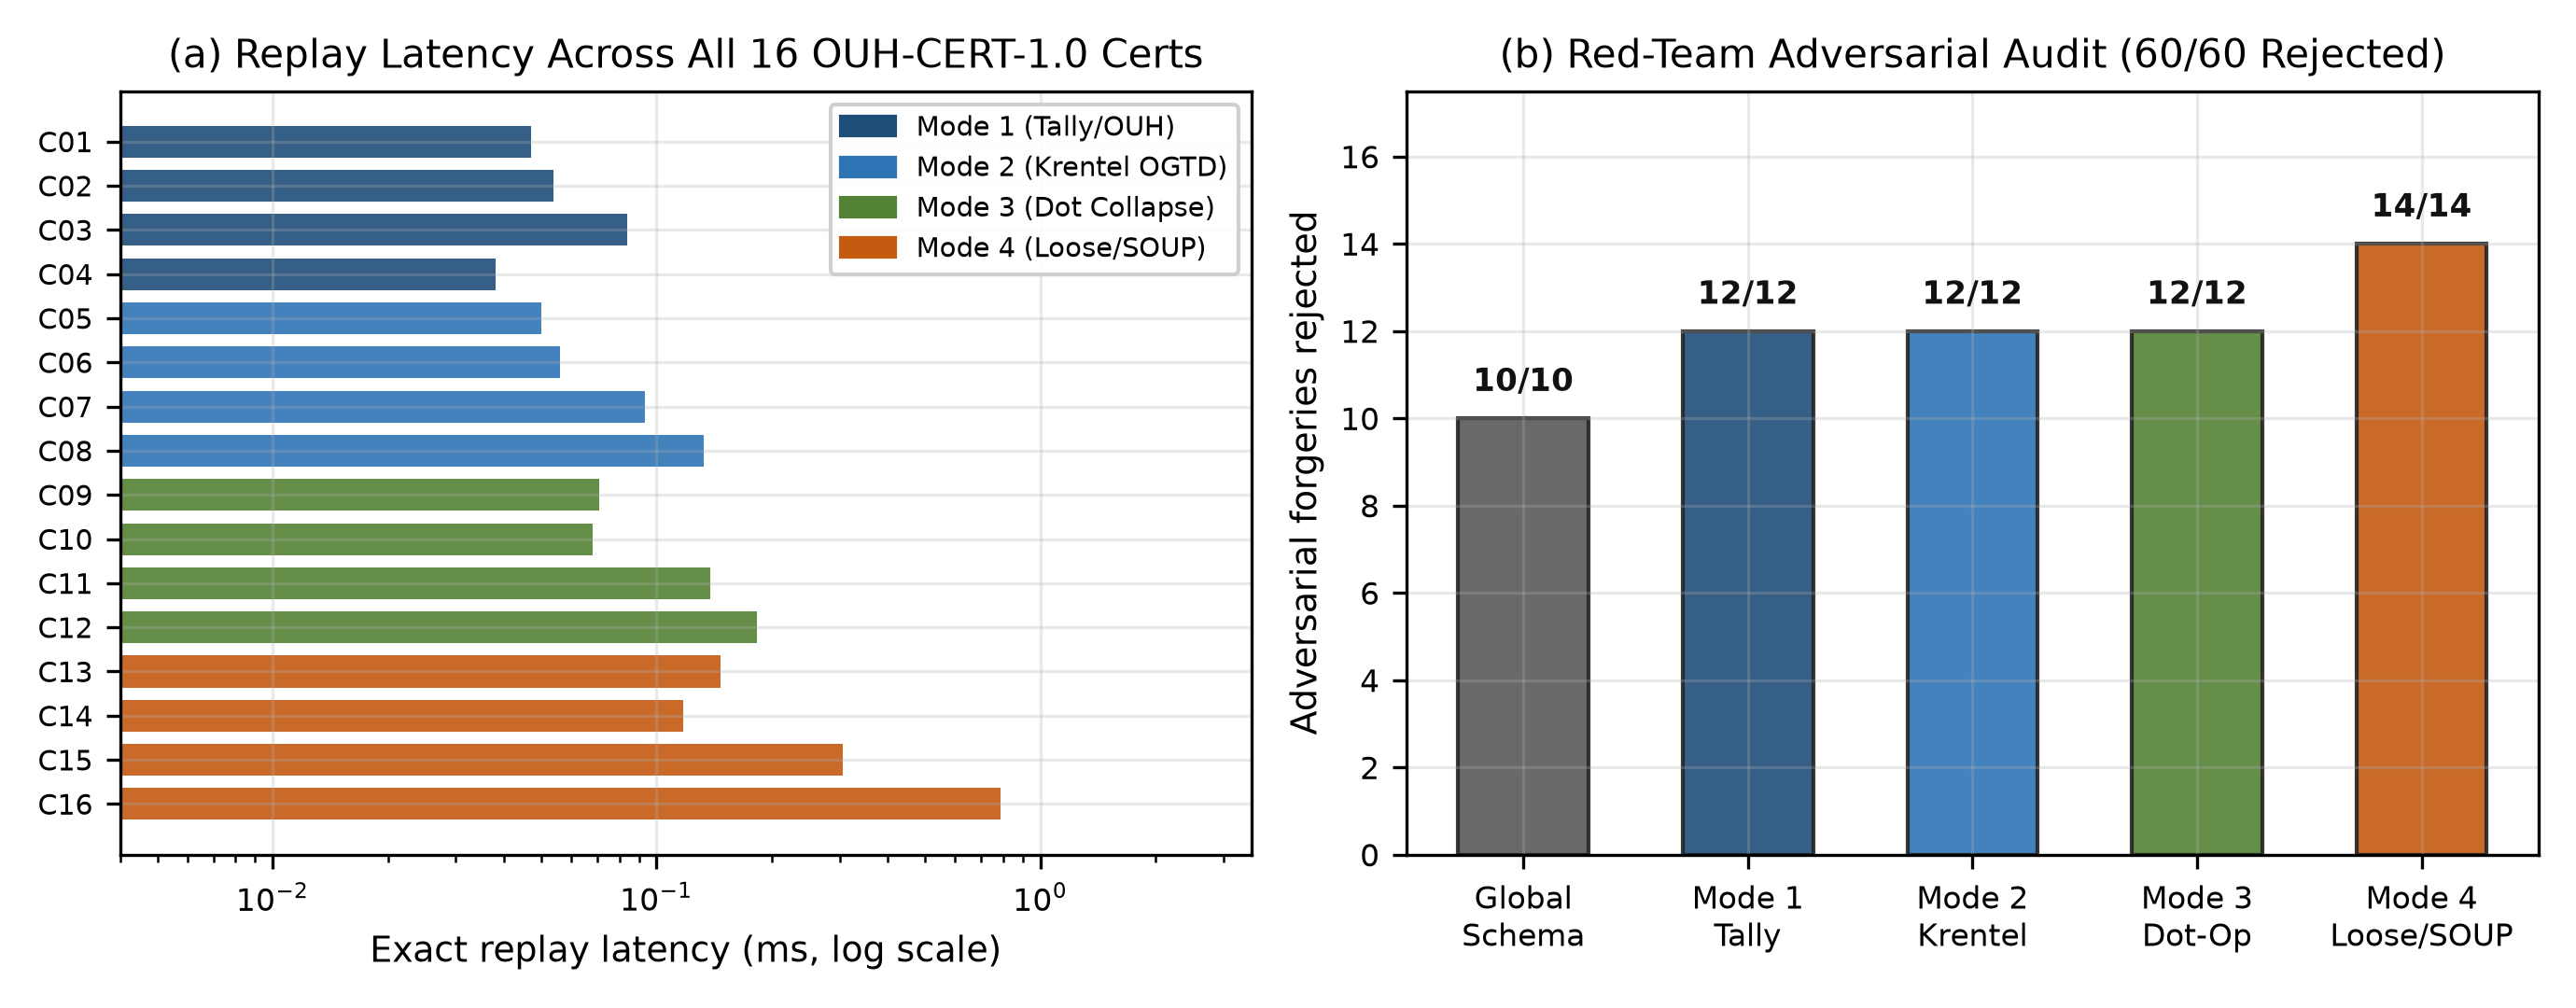
\includegraphics[width=\columnwidth]{../figures/fig3_certificate_replay_atlas.png}
  \caption{(a) Exact zero-float replay latency across all 16 canonical \texttt{OUH-CERT-1.0} certificates ($0.038$--$0.789\,\mathrm{ms}$). (b) Red-team adversarial audit rejecting 60/60 live forgery attacks across all modes.}
  \label{fig:atlas}
\end{figure}

\paragraph{Replay Atlas and Red-Team Audit (Fig.~\ref{fig:atlas}, Table~\ref{tab:replay}).}
All 16 canonical certificates replay in $0.038$--$0.789\,\mathrm{ms}$ with zero floats. Our adversarial suite (\texttt{tests/test\_suite.py}) tests 60 live forgery attacks---including float/bool type confusion, ambiguous or non-oblivious witnesses (e.g.\ two distinct $w_1 \neq w_2$ accepted in Mode~1), tampered Krentel prefix probes (Mode~2), vacuous or mismatched dot-collapse pairs (Mode~3), sensitive queries leaking into $\Pi_{\mathrm{out}}$ and non-complementary $\SOUP$ verifiers (Mode~4)---achieving \textbf{60/60 rejections} with zero bypasses.

\begin{table}[t]
\centering
\caption{Summary of all 16 canonical \texttt{OUH-CERT-1.0} certificates (representative witnesses) and 60/60 adversarial audit.}
\label{tab:replay}
\resizebox{\columnwidth}{!}{%
\begin{tabular}{@{}llcr@{}}
\toprule
Verification Mode & Concrete Certified Range & ms & Red-Team \\
\midrule
M1: Tally Census \& Extraction (4) & $h\le 12$ ($\binom{12}{6}{=}924{\to}1$), $n{\le}4,p{\le}6$, $0^5$ empty & 0.038--0.084 & 12/12 \\
M2: Krentel Lex-Max \& $\OUGTD$ (4) & $q\in[2,8]$, $|R|\in\{7,55,104\}$, $|\mathrm{Acc}_T|{=}1$ & 0.050--0.133 & 12/12 \\
M3: Dot-Operator Collapse (4) & $(n,p,r)\le(4,2,3)$, $32{\to}1$ unique $(w_n,v_N)$ & 0.068--0.183 & 12/12 \\
M4: Loose Query \& $\SOUP$ (4) & $2^5{=}32$ ext., $24/32$ insens., \texttt{1|wY} / \texttt{0|wZ} & 0.117--0.789 & 14/14 \\
Global Schema / Type / Bitstring & Float, bool-as-int, duplicate, bad bits & -- & 10/10 \\
\midrule
\textbf{Total (16 certs)} & \textbf{All 4 finite mechanisms of~\cite{hirsch2026oblivious}} & \textbf{0.038--0.789} & \textbf{60/60} \\
\bottomrule
\end{tabular}}
\end{table}

\section{Conclusion}
We delivered an 18-theorem zero-dependency Lean~4 kernel (11 zero-axiom theorems, 0~\texttt{Classical.choice}) with full formal specifications and the exact finite verifier \texttt{OUH-CERT-1.0} for the finite combinatorial core of Hirsch's input-oblivious unambiguous hierarchy collapses~\cite{hirsch2026oblivious}. Mechanizing uniform polynomial-time oracle Turing machines in Lean~4 to bridge these finite combinatorial lemmas to asymptotic complexity-class inclusions remains open.

\bibliographystyle{plain}
\bibliography{references}
\end{document}
